\documentclass[10pt,letterpaper]{article}
%\usepackage[a5paper]{geometry}%if printed as book
\usepackage[utf8]{inputenc}
\usepackage{amsmath}
\usepackage{amsfonts}
\usepackage{amssymb}
\usepackage[american,cuteinductors]{circuitikz}
\usepackage{hyperref}
\usepackage{booktabs}
\author{Scott Howard scott@scimpy.com}
\title{Scimpy:\\ \textbf{S}ound \textbf{C}ard based \textbf{I}mpedance \textbf{M}easurements in \textbf{Py}thon}
\date{Last Revision: \today}
\begin{document}
\maketitle
\tableofcontents
\section{Introduction}
test
\section{Usage}
test
\subsection{How to Connect Hardware}
Headphones are typically 32 ohms, so want to use 20 ohm resistor to protect circuits?

line out? does it have enough current?

line in: 600-47 kOhms (low impedance)
microphone, more sensitive but powered (need AC coupling?)
\subsection{How to Use the Software}
\subsubsection{Taking Data}
\subsubsection{Interpreting Data}
\section{Theory}
The mathematical description of loudspeakers is crucial to high-performance audio. This section describes and summarizes a common mathematical model, which is used by this program. This approach was developed by the pioneers Neville Thiele of the Australian Broadcasting Commission, and Richard H. Small of the University of Sydney, and the parameters are commonly known as the ``Thiele/Small Parameters."
\subsection{Impedance}\label{Impedance}
Speaker impedance represents how much voltage will be needed to drive 1~A of current  through the speaker voice coil. Higher resistance means that speaker response will drop, as it is harder to push current through it. Due to electrical, mechanical, and acoustical effects, impedance changes with frequency -- thus changing how the speaker sounds. If speaker impedance drops too low, more current will be needed from the amplifier. Over-driving the speaker amplifier risks distortion and overheating the amplifier. Additionally, passive cross-over circuits (i.e., what splits the signal to tweeter and woofer) are designed to work with loads whose impedance do not change with frequency; poor impedance matching reduces cross-over performance

However, this can be compensated for by adding an ``impedance matching" circuit right at the speaker. The circuit is designed such that the combined impedance of the speaker and circuit us the same for all frequencies, and thus avoiding signal distortion and amplifier damage.

Impedance circuits can be classified as active or passive. Active circuits are easier to design but are expensive and require additional power. Passive circuits are cheaper, but a well designed circuit will perform as well as an active system. However, designing such circuits requires specialized equipment and software. Thus the motivation for this project: develop a widely available, easy-to-use tool to measure impedance and provide impedance matching circuit designs.

Section~\ref{Impedance} will talk about how we describe and measure impedance, generally. Section~\ref{loudspeakers} will then build a model of loudspeaker impedance.
\subsubsection{Electrical Impedance}
Voltage ($V$) and current ($I$) are related to each other through the following expressions describing resistors (with resistance $R$), capacitors (with capacitance $C$), and inductors (with inductance, $L$):
\begin{align}\label{electrical_eqs}
V&=IR & V&=L\frac{\partial I}{\partial t} & I=C\frac{\partial V}{\partial t}
\end{align}

To understand their frequency response, we use generic time harmonic signals:
\begin{align}\label{timeharmonic}
V=V_0\cos(\omega t + \phi_{_V})&=\Re{ \left\{ \hat{V}e^{i\omega t}\right\} } &
I=I_0\cos(\omega t + \phi_{_I})&=\Re{ \left\{ \hat{I}e^{i\omega t}\right\} }
\end{align}

Where $\hat{V}(\omega)=V_0(\omega)e^{i\phi_{_V}(\omega)}$ and $\hat{I}(\omega)=I_0(\omega)e^{i\phi_{_I}(\omega)}$ are the phasor representation of voltage and current. Combining Equations~\ref{electrical_eqs} and \ref{timeharmonic} we can see that the phasor voltage and currents are proportional to each other by a factor of $Z$ for each of the circuit elements.
\begin{align}
\frac{\hat{V}}{\hat{I}}&=Z_R=R & Z_L&=i\omega L & Z_C&=\frac{1}{i\omega C}
\end{align}

Phasors allows us to easily calculate the relationship between voltage and current in complex circuits. For example, Figure~\ref{circuit1} can be represented using phasor sources and complex impedances as in Figure~\ref{circuit2}.

\begin{figure}
\centering
\begin{circuitikz}
  \draw (0,0)
  to[V=$V_0\cos(\omega t)$] (0,2) % The voltage source
  to[short] (1,2)
  to[short] (2,2)
  to[R=$R$] (2,0) % The resistor
  to[short] (0,0);
  \draw (2,2)
  to[short] (4,2)
  to[L=$L$] (4,0)
  to[short] (2,0);
  \draw (4,2)
  to[short] (6,2)
  to[C=$C$] (6,0)
  to[short] (4,0);
\end{circuitikz}
\caption{Example circuit}\label{circuit1}
\end{figure}

\begin{figure}
\centering
\begin{circuitikz}
  \draw (0,0)
  to[V=\mbox{$\hat{V}=V_0e^{i\omega t}$}] (0,2) % The voltage source
  to[short] (1,2)
  to[short] (2,2)
  to[generic=\mbox{$Z_R$}] (2,0) % The resistor
  to[short] (0,0);
  \draw (2,2)
  to[short] (4,2)
  to[generic=\mbox{$Z_L$}] (4,0)
  to[short] (2,0);
  \draw (4,2)
  to[short] (6,2)
  to[generic=\mbox{$Z_C$}] (6,0)
  to[short] (4,0);
\end{circuitikz}
\caption{Example circuit with complex impedances}\label{circuit2}
\end{figure}

Using standard circuit analysis, you can calculate the current coming out of the voltage source by treating each circuit element as if it was a resistor.
\begin{align}
Z=\left(\frac{1}{Z_R}+\frac{1}{Z_C}+\frac{1}{Z_L}\right)^{-1}
\end{align}
\begin{align}
\hat{I}=\hat{V}\left(\frac{Z_CZ_L+Z_RZ_L+Z_RZ_C}{Z_R+Z_C+Z_L}\right)=V_0e^{i\omega t}\left( \frac{L/C+i\left( -R/(\omega C)+\omega RL\right)}{R+i\left(\omega L - \omega/C\right)} \right)\label{complex_imp}
\end{align}

Current, $I$, can now be found by taking the real part of $\hat{I}$.

\subsubsection{Impedance Matching}
Our challenge is to design a circuit that makes the impedance constant for all frequencies. For example, a speaker has an impedance $Z=R+Z_0$, which represents a DC ($\omega=0$) resistance of $R$ and a frequency dependant impedance $Z_0$. to match impedance, a circuit with impedance $Z_1$ is added in parallel to the speaker, as depicted in Figure~\ref{simplespeaker}. The equivalent impedance is $Z=\frac{Z_1(R+Z_0)}{Z_1+Z_0+R}$. Setting $Z=R$ and solving for $Z_1$ yields:
\begin{align}\label{impmatching}
Z_1=R+\frac{R^2}{Z_0}
\end{align}

Equation \ref{impmatching} represents how we will design our impedance matching circuit. The circuit will consist of a resistor of resistance $R$ in series with a circuit that is the ``electric dual" of $Z_0$ scaled by $R^2$. The electric dual of a circuit with impedance $Z$ is defined as the circuit with impedance $Z'=1/Z$.

\begin{enumerate}
\item Develop a circuit model for $Z_0$ (and thus the dual circuit model for $Z'_0$)
\item Measure $R+Z_0$ as a function of frequency to extract $R$ and the values of the elements in the circuit model.
\end{enumerate}

\begin{figure}
\centering
\begin{circuitikz}[yscale=0.75]
  \draw (0,0)
  to[open,o-o] (0,4) % The voltage source
  to[short] (2,4)
  to[generic=\mbox{$\hat{Z}_1$}] (2,0) % The resistor
  to[short] (0,0);
  \draw (2,4)
  to[short] (4,4)
  to[R=$R$] (4,2)
  to[generic=\mbox{$\hat{Z}_0$}] (4,0)
  to[short] (2,0);
\end{circuitikz}
\caption{Speaker impedance matching}\label{simplespeaker}
\end{figure}

\subsubsection{Measuring Impedance}
Impedance testing is actually relatively straight forward. A function generator creates voltage to a circuit that has a resistor (of accurately known resistance $R_{test}$) in series with the speaker. The function generator creates a sinusoidal voltage with constant amplitude $V_0$ at different frequencies $\omega$. A volt meter measures the voltage across the test resistor, $v_r$, as a function of frequency $\omega$. The generic test system is described in Figure~\ref{imp_measure}. Speaker impedance can be found with the Equation~\ref{generic_imp}, below:
\begin{align}\label{generic_imp}
\hat{v}_s=\frac{ \hat{Z}_s V_0 }{ R_{test} + \hat{Z}_s } && \hat{i}_s=\hat{i}_r=\frac{\hat{v}_r}{R_{test}} && \hat{Z}_s=\frac{\hat{v}_s}{\hat{i}_s}=R_{test}\left( \frac{V_0}{\hat{v}_r} -1 \right)
\end{align}
All variables with carrots indicate complex numbers with a phase relative to the source, $V_0$.

Equation \ref{generic_imp} assumes the magnitude and phase of  $\hat{v}_1$ can be measured relative to the phase of the source with, for example, an oscilloscope locked in to the frequency and phase of the voltage source. If you don't have such a lock-in detection scheme (which few do), but do have time sensitive measurements (e.g., a sound card like we use in this project). You can rearrange Equation \ref{generic_imp} to be:
\begin{align}\label{generic_imp_2measure}
\hat{Z}_s=R_{test}\left( \frac{V_0 - \hat{v}_r}{\hat{v}_r}\right)=R_{test}\left( \frac{\hat{v}_s}{\hat{v}_r}\right)
\end{align}
which shows we need a another voltage meter to get $\hat{v}_s$. This is shown in Figure~\ref{imp_measure2}, and is the ciruit this project uses to find $\hat{Z}_s$ in Equation~\ref{generic_imp_2measure}).



Commonly, time-sensitive measurements are impractical as hobbyist typically only have multimeters, which can measure AC RMS. If only the RMS magnitude of AC voltage can be measured, then the magnitude of $Z$ can be found as in Equation~\ref{generic_imp_mag}.
\begin{align}\label{generic_imp_mag}
\hat{\left|Z_s\right|}=\frac{\left| v_s \right| R_{test}}{\left| v_r \right|}
\end{align}

It is important to note how Equation~\ref{generic_imp_mag} differs from many hobbyist impedance measurement techniques (incorrectly: $\left| Z_s \right| = R\left(\frac{ \left| V_0 \right|}{\left| v_r \right|}-1\right) $) which ignores the fact that phases of each of the voltages are not the same!

\begin{figure}
\centering
\begin{circuitikz}
  \draw (0,0)
  to[V=\mbox{$V_0\cos(\omega t)$}] (0,2) % The voltage source
  to[short] (1,2)
  to[R=$R_{test}$,i=$\hat{i}_r$,v=$\hat{v}_r$,o-o] (3,2) % The resistor
  to[short] (4,2)
  to[generic=\mbox{$\hat{Z}_s$},v=$\hat{v}_s$,i=$i_s$] (4,0)
  to[short] (0,0);
  \draw (1,2)
  to[short] (1,1)
  to[voltmeter] (3,1)
  to[short] (3,2);
\end{circuitikz}
\caption{Typically described speaker impedance measurement (requires voltmeter to be locked-in to the source phase)}\label{imp_measure}
\end{figure}

\begin{figure}
\centering
\begin{circuitikz}
  \draw (0,0)
  to[V=\mbox{$V_0\cos(\omega t)$}] (0,2) % The voltage source
  to[short] (1,2)
  to[R=$R_{test}$,i=$\hat{i}_r$,v=$\hat{v}_r$,o-o] (3,2) % The resistor
  to[short] (4,2)
  to[generic=\mbox{$\hat{Z}_s$},v=$\hat{v}_s$,i=$i_s$] (4,0)
  to[short] (0,0);
  \draw (1,2)
  to[short] (1,1)
  to[voltmeter] (3,1)
  to[short] (3,2);
  \draw (4,2)
  to[short,o-] (5.5,2)
  to[voltmeter, mirror] (5.5,0)
  to[short,-o] (4,0);
\end{circuitikz}
\caption{Speaker impedance matching (this project, no lock-in required)}\label{imp_measure2}
\end{figure}


Once $\hat{Z}$ or $\left| \hat{Z} \right|$ is found for different frequencies $\omega$, you can fit the data to the models in Section~\ref{loudspeakers} to extract the values needed to make the impedance matching circuit.

\subsubsection{Crossover Circuits and Impedance}
Cross-over circuits are needed to separate the sound signal into high and low frequency components. Ideally for dipole speakers, you want a ``switch" that sends low frequency below some cross-over frequency $\omega_c$ only to the woofer and higher frequencies only to the tweeter. Practically, some leakage will occur in separating the signals such that some low frequencies will end up at the tweeter, and high at the woofer.  These negative effects define the engineering problem.

Cross-over circuits are either classified as active (powered) or passive (unpowered). \textit{Active cross-overs} use operational amplifiers (op amps) that can drive loads with complex $\hat{Z}$ uniformly across all frequencies and thus do not need impedance matching circuits. However, they tend to be a bit complicated, expensive, and require additional power. \textit{Passive cross-overs} are cheaper, simpler, and don't require extra power -- but do require extra care in design to achieve the same same theoretical performance as active cross-overs. Since we have the tools to properly design cross-overs, we will consider passive cross-overs.

The first step is to impedance match the speaker, which we have done by measuring the impedance, extracting the required component values, and using an impedance matching circuit. Next, the simplest electric filter is an inductor or a capacitor in series with a resistor to make a low-pass and high-pass filter, respectively, as in Figure~\ref{filters}.

\begin{figure}
\centering
\begin{circuitikz}
  \draw (0,0)
  to[open,v^>=$v_i$,o-o] (0,2) % The voltage source
  to[short] (1,2)
  to[generic=$\hat{Z}$] (3,2) % The resistor
  to[short] (4,2)
  to[R=$R_S$,v=$\hat{v}_o$,o-o] (4,0)
  to[short] (0,0);
\end{circuitikz}
\caption{First order filter}\label{filters}
\end{figure}

The transfer function ($\hat{H}$, the ratio of output to input voltage) can be found for $\hat{Z}=i\omega L$ and $\hat{Z}=\frac{1}{i\omega C}$
\begin{align}
\hat{H}_{LP}(\omega)=\left( {1+\frac{i\omega L}{R}} \right)^{-1}
=\left( {1+\frac{i\omega}{\omega_c}} \right)^{-1}
&=\left( {1+\frac{\omega^2}{ \omega_c^2}}\right)^{-\frac{1}{2}} e^{\tan^{-1}\left( \frac{\omega}{\omega_c}\right)}\\
\hat{H}_{HP}(\omega)
=\left( {1+\frac{1}{i \omega R C}} \right)^{-1}
=\left( {1+\frac{\omega_c}{i \omega}} \right)^{-1}
&=\left( {1+\frac{\omega_c^2}{\omega^2 }}\right)^{-\frac{1}{2}} e^{\tan^{-1}\left( \frac{\omega_c}{\omega}\right)}
\end{align}

$L$ and $C$ are picked for a given cross-over frequency such that $L=\frac{R}{\omega_c}$ and $C=\frac{1}{R\omega_c}$. Note that the sum of both speaker outputs $\hat{H}_{LP}(\omega)+\hat{H}_{HP}(\omega)~=~1$ for all frequencies! That means that the signal is transferred perfectly in amplitude (volume) and phase (audible delay) at every frequency. However, each driver demonstrates a group phase delay ($\partial \phi / \partial \omega$) in the pass-bands, so how can it appear to have zero-phase? Well, it's a bit of a trick in that the system ``uses"  \textit{both} speakers to correct for this variable delay as a function of frequency. Low frequencies coming from the woofer have small delay (phase), while those low frequencies in the tweeter have a lot of delay. As frequency increases, woofer delay increases and tweeter delay decreases. The apparent phase (delay) is unchanged. This is not ideal as it relies on driving your tweeter lower than designed (risking overheating and damage) and your woofer higher than intended (excited standing waves/nodes within the woofer driver which degrades sound quality). Therefore, high-order filters are preferred.

High order filters (i.e., ones that separate tweeter and woofer signals better) can be used, but requires more parts. See, for example, Linkwitz-Riley (LR) filters for a high-order filter. The LR2 filter design is shown in Figure~\ref{LRfilters}. Choosing $Z_1=Z_2$ and $R_s=R_1$, you can calculate transfer functions in the Maxima computer algebra system (left for the reader):
\begin{verbatim}
ZL1:%i*w*L1;
Zsub:((R1+ZL1)^(-1)+1/R1)^(-1);
transferfunc:Zsub/(Zsub+ZL1);
(declare(w,mainvar),ratexpand(transferfunc));
\end{verbatim}

You can see that the LR2 filter has many positive features compared to our simple filter:
\begin{itemize}
\item Faster roll-off (12 dB/octave versus 6 dB/octave) - better separation of frequencies to protect the drivers
\item Phase is flat (low group delay) in the pass-bands. There is, however, some group delay around cross-over.
\item Constant phase offset between woofer \& tweeter for all frequencies. Offset is 180$^\circ$, so you need to to wire one of the drivers backwards (negative polarity).
\item Like our simple system, choose $L=R/\omega_c$ and $C=1/(\omega_c R)$.
\end{itemize}


\begin{figure}
\centering
\begin{circuitikz}
  \draw (0,0)
  to[open,v^>=$v_i$,o-o] (0,2) % The voltage source
  to[short] (1,2)
  to[generic=$\hat{Z_1}$] (3,2) % The resistor
  to[R=$R_1$,] (3,0)
  to[short] (0,0);
  \draw (3,2)
  to[generic=$\hat{Z_2}$] (5,2)
  to[R=$R_S$,v=$\hat{v}_o$,o-o] (5,0)
  to[short] (3,0);  
\end{circuitikz}
\caption{Linkwitz-Riley Second Order Filter (LR2)}\label{LRfilters}
\end{figure}




\subsubsection{Correct for difference in efficiency L-pad}

\subsection{How Do Loudspeakers Work?}\label{loudspeakers}
A loudspeaker converts electrical signals to sound waves by using the signal electrical voltage to drive a current which applies a force on a speaker membrane that in turn pushes a volume air. This pushed volume of air propagates as a sound wave to the listener.

To understand this process, we will break down the electrical, mechanical, and acoustical systems individually. We will also describe how each are connected. From the individual system models and our understanding of how they are connected, we will finally integrate them in to a complete single model which can be used to describe how loudspeakers work.
\subsubsection{Electrical Model}
A loudspeaker driver is fundamentally a system that translates electrical current to motion. Current through a coil of wires (called the voice coil) interacts with a permanent magnet, as described in Figure~\ref{speaker_diagram}\footnote{By Iain, png by Rohitbd (SVG version of en:Image:Speaker cross section.PNG) [CC-BY-SA-3.0 (http://creativecommons.org/licenses/by-sa/3.0/)], via Wikimedia Commons}. Wire, itself, is a resistor; when coiled a wire a an inductor; and the time varying magnetic field created by and inductor induces ``eddy currents" in nearby conductors which act as a resistor in parallel with the inductor. This electrical current is then can be coupled to the mechanical vibrations (discussed in Section~\ref{mechanical_section}). The electrical model is thus described in Figure~\ref{electrical_model}. Where $R_{vc}$ is the DC resistance of the voice coil, $L_{vc}$ is the inductance of the voice coil, $\hat{Z}_e$ is the electrical impedance equivalent to the mechanical impedance due to the electrical-mechanical coupling, and $R_{eddy}$ is the effective resistance due to eddy currents which is typically very high and frequently ignored in models. Finally, the current $i_e$ is the current that couples to mechanical motion described by $\hat{Z}_e$ as described in Section~\ref{mechanical_section}.

\begin{figure}
\centering
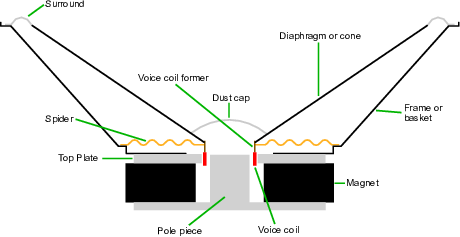
\includegraphics[height=0.25\textheight]{Speaker-cross-section.png}
\caption[Loudspeaker Driver]{Loudspeaker Driver}
\label{speaker_diagram}
\end{figure}

\begin{figure}
\centering
\begin{circuitikz}
  \draw (0,0)
  to[open,v^>=$v_i$,o-o] (0,2) % The voltage source
  to[R=$R_e$] (2,2) % The resistor
  to[L=$L_e$,mirror] (4,2)
  to[short] (5,2)
  to[generic=$\hat{Z_e}$,i=$i_e$] (5,0)
  to[short] (0,0);
  \draw (2,2)
  to[short] (2,3)
  to[R=$R_{eddy}$] (4,3)
  to[short] (4,2);
\end{circuitikz}
\caption{Electrical Model}\label{electrical_model}
\end{figure}


\subsubsection{Mechanical Model}\label{mechanical_section}
Electric current is coupled to mechanical motion through the Loretnz Force equation:
\begin{align}
\mathbf{F}=Q\mathbf{E}+Q\mathbf{v}\times \mathbf{B}=Q\mathbf{E}+Q\ell\mathbf{I}\times \mathbf{B}
\end{align}
Where $F$ is force, $Q$ is charge, $v$ is velocity of the charge, and $B$ is the magnetic field (i.e., the length of the coil), $\ell$ is length of the wire in the field, and $I$ is the current. When current is moving in the wire, it exerts a force of
\begin{align}
F=IB\ell\label{force_current}
\end{align}
When a wire moves perpendicular to a magnetic field, carriers inside the wire feel a force of $F_B=QvB$. This force pushes electrons to one end of the wire, which creates a Coulomb force of $F_E=QE$. These two forces sum to zero, so $vB=-E$. This allows us to connect voltage across the coil, $V$, to velocity, $v$:
\begin{align}
V=-\int E\,d\ell=\int vB\,d\ell=vB\ell\label{velocity_potential}
\end{align}
From Equations~\ref{force_current} and \ref{velocity_potential} this description, electrical impedance can be found in terms of force $F$ and $v$ in a mechanical system:
\begin{align}
\hat{Z}_e=\frac{V}{I}=\frac{v}{F}\left(B\ell\right)^2
\end{align}

To continue with our model, we need to find the relationship between $v$ and $F$, so we turn to Newton's law of motion and Hook's law for a dampened mass on a spring:
\begin{align}
\sum F&=M_{md}\frac{d^2x}{dt^2}\\
F-\frac{1}{C_{ms}}x&=M_{md}\frac{d^2x}{dt^2}+R_{ms}\frac{dx}{dt}\\
F&=M_{md}\frac{dv}{dt}+R_{ms}v+\frac{1}{C_{ms}}\int v\,dt\\
F(\omega)&=i\omega M_{md}v+R_{ms}v+\frac{1}{i\omega C_{ms}}v\label{force_equation}
\end{align}
where $M_{md}$ is the mass of the diaphragm and coil, $C_{ms}$ is the compliance of the suspension (i.e., $1/k$ of Hooke's Law), and $R_{ms}$ represents the coefficient of friction (mechanical resistance to motion). From Equation~\ref{force_equation}, you can see that we can actually model mechanical systems as electrical circuits. In such a circuit,  voltages represent force, current represents velocity, inductance is mass, electrical resistance is mechanical resistance, and capacitance is compliance. Mechanical impedance, is thus:
\begin{align}
\hat{Z}_m&=\frac{F}{v}\\
\hat{Z}_e &= \hat{Z}_m^{-1} (B\ell)^2\label{mech_imp_dual}
\end{align}
Equation~\ref{mech_imp_dual} shows that if we represent our mechanical system as a mechanical circuit and find the mechanical impedance, the equivalent electric circuit is the dual of the mechanical circuit scaled by $(B\ell)^2$.

The mechanical system in Equation~\ref{force_equation} describes the speaker in vacuum, that is without interacting with air. The driver will push a volume of air to generate sound, and thus is an additional complex component in our circuit. Therefore the complete mechanical circuit is described in Figure~\ref{mechanical_model}.
\begin{figure}
\centering
\begin{circuitikz}
  \draw (0,0)
  to[open,v^>=$F$,o-o] (0,2) % The voltage source
  to[L=$M_{md}$] (2,2) % The resistor
  to[R=$R_{ms}$] (4,2)
  to[C=$C_{ms}$] (6,2)
  to[generic=$\hat{Z_m}$,i=$v$] (6,0)
  to[short] (0,0);
\end{circuitikz}
\caption{Mechanical Model}\label{mechanical_model}
\end{figure}

\subsubsection{Acoustical Model}
From Section~\ref{mechanical_section}, we found a way to find the velocity the diaphragm will move as a function of input current. The moving diaphragm will push air and create a pressure wave, which is what we will hear. The speaker diaphragm pushes the following $V$ of air per second:
\begin{align}
Q=S_dv\label{eq:volume_velocity}
\end{align}
Where $Q$ is the volume velocity, $v$ is diaphragm velocity as found in Section~\ref{mechanical_section}, and $S_d$ is the area of the driver diaphragm. Also, it is possible to convert between mechanical and acoustic impedances by using the speaker diaphragm area $S_d$:
\begin{align}
Z_m=\frac{F}{v}=\frac{pS_d}{Q/S_d}= S_d^2 Z_a\label{eq:acoustic-to-mech_imp}
\end{align}

When mounted in a speaker enclosure, the air pushed/pulled from the front of the diaphragm radiates as sound waves while the air pushed/pulled from the back of the driver is shielded from the listener. This is because the sound waves from the back are perfectly out of phase from the front, and thus will lead to audio nulls in the room.

To stop this interference, the air pushed/pulled from the back of the driver is typically enclosed in a box. Through some acoustic tricks, one can invert the phase of the rear acoustic waves by the use of a ``port" or "bass reflex" which is essentially a tube opening up to the space the inside of the speaker enclosure. See Figure~\ref{bass_reflex} \footnote{By Rohitbd, original by Melancholie.\\
CC-BY-SA 3.0, https://en.wikipedia.org/w/index.php?curid=2745689}.

\begin{figure}
\centering
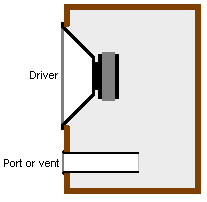
\includegraphics[height=0.25\textheight]{Bass_reflex_spk.png}
\caption{Bass Reflex Speaker or Vented Speaker Enclosure}\label{bass_reflex}
\end{figure}

We will consider this vented enclosure as our model since it is an extremely common enclosure  and the model can be easily adapted for other enclosures. First, we must find what the change in pressure $p$ is caused by $Q$. We know that pressure is increased per percent change in gas volume in the box $V_B$ by a factor of compressibility$^{-1}=\rho c^2$ :
\begin{align}
p=\rho c^2 \frac{\Delta V_B}{V_B}=\rho c^2 \frac{\int Q_B dt}{V_B}\\
\hat{p}=\frac{\rho c^2}{i\omega V_B}\hat{Q}_B=\frac{1}{i\omega C_{ab}}\hat{Q}_B\label{acoustic_compression}
\end{align}
where $Q_B$ is the volume velocity in to the box, $\rho$ is gas density, $c$ is the speed of sound, and $C_{ab}=\frac{V_B}{\rho c^2}$ is the acoustic capacitance of the box.

This increase of pressure inside the box will cause air flow in 
the port or vent, and acoustic radiation away from the vent. This air flow in a vent with area $A_v$, length $\ell_v$, volume $V_v$ will cause a pressure drop due to Newton's Law:
\begin{align}
F&=m\frac{dv}{dt}+\frac{\mu V_v}{\kappa} v\\
p&=\rho \frac{\ell_v}{A_v}\frac{dQ_v}{dt}+\frac{\mu \ell_v}{\kappa A} v\\
\hat{p}&=i\omega\rho \frac{\ell_v}{A_v}\hat{Q}_v+\frac{\mu \ell_v}{\kappa A_v} \hat{Q}_v\\
\hat{p}&=i\omega L_{av} \hat{Q}_v+R_{av} \hat{Q}_v \label{acoustic_flow}
\end{align}
where the second term is Darcy's law that describes $Q$ in a porous medium \textit{permeability} of $\kappa$ and viscosity $\mu$.

In theory, every time there is flow, acoustic inductance, resistance, and capacitance is present. Therefore, a generic element follows both Equation~\ref{acoustic_compression} and \ref{acoustic_flow}:
\begin{align}
\hat{p}&=i\omega L \hat{Q}+R \hat{Q} +\frac{1}{i\omega C}\hat{Q}
\end{align}
However, only one or two of the terms will typically dominate. To determine which to use, each can be calculated (effectively determining the Reynolds number). General rules to determine which effects are present are described in Table~\ref{table:acoustic}.


\begin{table}
\centering
\renewcommand{\arraystretch}{1.5}
\begin{tabular}{@{} l p{.25\textwidth} p{.5\textwidth} @{}}
\toprule
Term & Description & Usage \\
\midrule
$L = \frac{\rho \ell}{A}$ & Air flowing through open space & Speaker vent/port ($L_{av}$)  \\ 
$R = \frac{\mu \ell }{\kappa A}$ & Air flowing through a porous or a highly scattering path &
Air leaking out the box ($R_{al}$); \newline 
Air flowing through acoustic filling material inside the box ($R_{ab}$)\\
$C = \frac{V}{\rho c^2}$ & Air compressing inside an enclosure & Air compression in the box ($C_{ab}$)\\
\bottomrule
\end{tabular}
\caption{Guide to Acoustic Impedance Terms}\label{table:acoustic}
\end{table}

To account for air leakage out of the box, we can use Table~\ref{table:acoustic} to describe the volume of air to flow leaking out of the box each second:
\begin{align}
\frac{p}{R_{al}} = Q_l
\end{align}


Finally, we can get to acoustic radiation... that is sound! For this, we will find the relationship between volume velocity $Q$ and pressure $p$ at a radiation point (driver or bass vent). To do this, we start with the pressure wave equation:
\begin{align}
\left(\nabla^2-\frac{1}{c^2}\frac{\partial^2}{\partial t^2}\right)p=0
\end{align}
and assume a spherical wave solution of the form:
\begin{align}
p=\Re \left\{ \frac{K}{r} e^{i(\omega t - k r)} \right\}
\end{align}
where $K$ is an unknown constant and $k=\omega/c=2\pi/\lambda$ (i.e., the spatial frequency of the wave). We know that at the port, we have volume velocity $Q_0$, so we need to find $K$ at the boundary. The easiest way to do this is to assume $Q=Q_0$ when $r$ is equal to the radius of your opening $a$. That basically places a spherical monopole in your opening. Moving on assuming a time harmonic volume velocity $Q=\Re\left\{\hat{Q}_0e^{i\omega t}\right\}$ we can find $Q$ from the surface of our spherical monopole with radius $a$:
\begin{align}
Q_a=Av_a(t)=\frac{4\pi a^2}{2} v_a(t) = \hat{Q}_0e^{i\omega t}
\end{align}
where $Q_0$ is the volume velocity inside the port. The velocity at radius $a$ from the center of the port is thus:
\begin{align}
v_a=\frac{1}{2\pi a^2} \hat{Q}_0 e^{i\omega t}
\end{align}


%
%\begin{align}
%\frac{\partial m}{\partial t} &=-\oint \rho \mathbf{v}\cdot d\mathbf{s}\\
%\int \frac{\partial \rho}{\partial t} dV &=-\int \boldsymbol{\nabla} \cdot \rho \mathbf{v}\, dV\\
%\frac{\partial \rho}{\partial t}+ \boldsymbol{\nabla} \cdot \rho \mathbf{v}&=0\\
%\end{align}
%and linearizing  $\rho=\rho_0+\rho'$ where $\rho'$ is a small deviation from equilibrium $\rho_0$, (i.e., $\rho_0\gg \rho'$)
%\begin{align}
%\frac{\partial \rho}{\partial t}+ \rho_0 \boldsymbol{\nabla} \cdot \mathbf{v}&=0\\
%\end{align}
%Density is linearly proportional to pressure, so considering only the $r$ direction


To make the connection between pressure and velocity, we can look to conservation of momentum. Momentum conservation says that the rate of momentum increase is equal to the force density $f$ (N/m$^3$) on a fluid.
\begin{align}
F&=m\frac{dv}{dt}\\
\int f dV &= \int \rho \frac{dv}{dt} dV\\
f&=\frac{\partial}{\partial t} (\rho v) \\
-\nabla p &= \rho \frac{\partial}{\partial t}\left( \hat{v}e^{i\omega t } \right)\\
\frac{ikK}{r} e^{i(\omega t - k r)} + \frac{K}{r^2} e^{i(\omega t - k r)} &=\rho i\omega \hat{v}e^{i\omega t}\\
\frac{kK}{\omega \rho r} e^{-ikr} - \frac{iK}{\omega \rho r^2} e^{-ikr} &= \hat{v}\label{solve_for_K}
\end{align}
We now evaluate Equation~\ref{solve_for_K} at $r=a$:
\begin{align}
\frac{kr\,K}{\omega \rho r^2} e^{-ikr} - \frac{iK}{\omega \rho r^2} e^{-ikr} &= \frac{1}{2\pi a^2} \hat{Q}_0\\
K &= \frac{\omega\rho}{2\pi({ka-i})} \hat{Q}_0e^{ika}
\end{align}
Therefore:
\begin{align}
p&=\frac{\omega\rho \hat{Q}_0}{2\pi r(ka-i)} e^{i(\omega t - k (r-a))}\\
\hat{Z}&=\frac{\hat{p}}{\hat{Q}}|_{r=a}=\frac{\omega \rho}{2\pi a(ka-i)}=\frac{\omega^2 \rho }{2\pi c(k^2a^2+1)}+\frac{i \rho }{2\pi ka(k^2a^2+1)}
\end{align}
Now we consider $ka\approx0$ since $a \ll \lambda$:
\begin{align}
\hat{Z}_{rad}&=\frac{\omega^2 \rho }{2\pi c}
\end{align}


We now have all the tools to model the acoustic system as a circuit. When the speaker driver moves with velocity $v$ (as determined in Section~\ref{mechanical_section}, It will create a $Q_d=v_dS_d$. This $Q_d$ radiates as sound and also drives air into the enclosure box $Q_b$. The increased volume of air in the box increases the pressure in the box. Increased pressure drives air to leak out of the box; and the box increase in box pressure causes flow and radiation out of the vented port. This complete model is described in Figure~\ref{acoustic_model}. The forward speaker radiation $p_f$ is in reverse polarity to indicate the radiation is $180^\circ$ out of phase from $Q_d$ since $Q_d$ is defined as positive when pushing air in to the enclosure. $R_{ab}$ is included to account for pressure loss due to filling material in the enclosure. Figure~\ref{acoustic_model_simple} shows a commonly employed simplified model; we will see in Section~\ref{sec:combined_model} that several terms will be able to be combined to yield this simplified model.


\begin{figure}
\centering
\begin{circuitikz}[yscale=.75]
  \draw (0,0)
  to[open,v^>=$p_i$,o-o] (0,4) % The voltage source
  to[short,i=$Q_d$] (1,4)
  to[R=$Z_{rad}$,v>=$p_{f}$] (3,4)
  to[short] (4,4)
  to[C=$C_{AB}$,i>^=$Q_{ab}$] (4,2)
  to[R=$R_{AB}$] (4,0)
  to[short] (0,0);
  \draw (4,4)
  to[short] (6,4)
  to[R=$R_{AL}$,i>^=$Q_{al}$] (6,0) % The resistor
  to[short] (4,0);
  \draw (6,4)
  to[R=$R_{av}$] (8,4)
  to[L=$L_{av}$,i>^=$Q_{av}$] (8,2)
  to[R=$Z_{rad}$,v=$p_{r}$] (8,0)
  to[short] (6,0);
\end{circuitikz}
\caption{Acoustic Circuit Model}\label{acoustic_model}
\end{figure}

\begin{figure}
\centering
\begin{circuitikz}
  \draw (0,2)
  to[open,v^>=$p_i$,o-o] (0,4) % The voltage source
  to[short,i=$Q_d$] (2,4)
  to[C=$C_{AB}$,i>^=$Q_{ab}$] (2,2)
  to[short] (0,2);
  \draw (2,4)
  to[short] (4,4)
  to[R=$R_{AL}$,i>^=$Q_{al}$] (4,2) % The resistor
  to[short] (2,2);
  \draw (4,4)
  to[short] (6,4)
  to[L=$L_{av}$,i>^=$Q_{av}$] (6,2)
  to[short] (4,2);
\end{circuitikz}
\caption{Common Simplified Acoustic Circuit Model}\label{acoustic_model_simple}
\end{figure}

\textbf{bass reflect out of phase!? yes/no!?}

\subsubsection{Combined Model}\label{sec:combined_model}
In this section, we will combine our models into a single model, then show how measurements can extract values for each of the components.

First, we combine the acoustic model with the mechanical using Equations~\ref{eq:volume_velocity} and \ref{eq:acoustic-to-mech_imp} to generate Figure~\ref{mech-acoustic_model}.

\begin{figure}
\centering
\begin{circuitikz}[yscale=.75]%[scale=VALUE,transform shape] to shrink in 2D more
  \draw (-2,0)
  to[open,v^>=$F$,o-o] (-2,4) % The voltage source
  to[L=$M_{md}$] (0,4)
  to[R=$R_{ms}$] (1.5,4)
  to[C=$C_{ms}$] (2.5,4)
  to[R=$S_d^2 Z_{rad}$] (4,4)
  to[short] (4,4)
  to[C=$S_d^2 C_{ab}$] (4,2)
  to[R=$S_d^2 R_{ab}$] (4,0)
  to[short] (-2,0);
  \draw (4,4)
  to[short] (6,4)
  to[R=$S_d^2 R_{al}$] (6,0) % The resistor
  to[short] (4,0);
  \draw (6,4)
  to[R=$S_d^2 R_{av}$] (8,4)
  to[L=$S_d^2 L_{av}$] (8,2)
  to[R=$S_d^2 Z_{rad}$] (8,0)
  to[short] (6,0);
\end{circuitikz}
\caption{Mechanical-Acoustic Circuit Model}\label{mech-acoustic_model}
\end{figure}

Next, we remember Equation~\ref{mech_imp_dual} to convert from mechanical impedances to electrical $Z_e=(BI)^2Z_m^{-1}$. That means we have to find the dual of Figure~\ref{mech-acoustic_model} and place that circuit in Figure~\ref{electrical_model}.

\begin{figure}
\centering
\begin{circuitikz}[xscale=.75]%[scale=VALUE,transform shape] to shrink in 2D more
  \draw (-2,0)
  to[open,v^>=$v_0$,o-o] (-2,2)
  to[R=$R_e$] (0,2)
  to[L=$L_e$] (2,2)
  to[C=$C_{mes}$,mirror] (2,0)
  to[short] (-2,0);
  \draw (2,2)
  to[short] (4,2)
  to[R=$R_{es}$] (4,0)
  to[short] (2,0);
  \draw (4,2)
  to[short] (6,2)
  to[L=$L_{ces}$] (6,0)
  to[short] (4,0);
  \draw (6,2)
  to[L=$L_{ceb}$] (8,2)
  to[R=$R_{el}$] (10,2)
  to[C=$C_{lev}$, mirror] (10,0)
  to[short] (6,0);
  \draw (10,2)
  to[short] (12,2)
  to[R=$R_{ev}$] (12,0)
  to[short] (10,0);
  \draw (6,2)
  to[short] (6,3)
  to[R=$R_{eb}$] (8,3)
  to[short] (8,2);
  \draw (0,2)
  to[short] (0,3)
  to[R=$R_{eddy}$] (2,3)
  to[short] (2,2);
\end{circuitikz}
\caption{Mechanical-Acoustic Circuit Model}\label{elec-mech-acoustic_model}
\end{figure}

to R=$S_d^2 R_{ab}$  (4,0)


\hrule

\textbf{when there is no box, $Q_b=Q_l=0$, load is inductive and added to $M_ms$}

should i make inductors all value of M?

\subsubsection{Monopole Radiation}


%                                         #1 + ZL2 w - R 1i
%---------------------------------------------------------------------------------------------------
%                                 2                2                       3                    4
%ZL1 w - R 1i + ZL2 w + C1 R ZL1 w  1i + C2 R ZL1 w  1i + #1 - C1 ZL1 ZL2 w  - C1 C2 R ZL1 ZL2 w  1i
%
%where
%
%                   2
%   #1 == C2 R ZL2 w  1i
 
\end{document}